\chapter{Methode}
Um diese Anforderungen zu erfüllen, haben wir das Tracking-By-Detection Paradigma übernommen, eine effektive Methode für Aufgaben des Multi-Object-Tracking (MOT), wobei wir YOLOv8 \cite{redmon2016look} als Detector und BoT-SORT \cite{aharon2022botsort} als Tracker verwenden. Zur Implementierung dieses Systems nutzen wir das Ultralytics Framework \cite{yolov8_ultralytics}. Dieses Framework bietet nützliche Funktionen für das Training eines end-to-end YOLO-Modells und die nahtlose Integration des Trackers in unser System.

Das Tracking-by-Detection Paradigma \ref{fig:part01:tracing-by-detection} basiert auf der Verwendung eines Object-Detection Modells als Detector, das dazu dient, Objekte in einem Bild zu erkennen und ihre Bounding Boxes zurückzugeben. Ein Tracking Algorithmus kommt ebenfalls zum Einsatz, um die Informationen aus den Bounding Boxes, die vom Detector bereitgestellt werden, zu nutzen und diesen Bounding Boxes eine konsistente Objekt-ID über die gesamte Dauer des Videos zuzuweisen.

\begin{figure}[htbp]
 \centering
 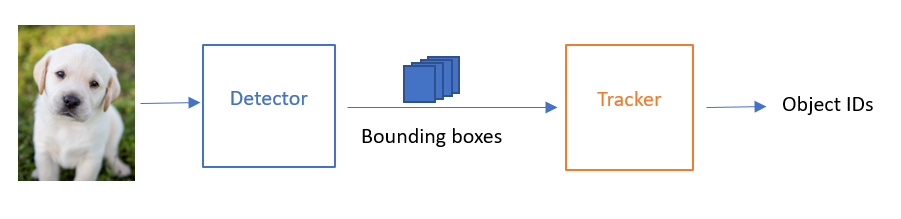
\includegraphics[width=1\textwidth]{gfx/tracking_by_detection.png}
 \caption{Darstellung des tracking-by-detection Paradigmas. Quelle: Eigene Quelle}
 \label{fig:part01:tracing-by-detection}
\end{figure}

\section{Object detection}
\label{sec:intro:motivation}
Als Detector verwenden wir YOLO, das ein Echtzeit-Objekterkennung-Modell ist und auf \acs{CNN} basiert. Es wurde entwickelt, um End-to-End-Training zu ermöglichen und Echtzeitverarbeitungsgeschwindigkeiten bei gleichzeitig hoher durchschnittlicher Präzision zu liefern. YOLO hat aufgrund seiner hohen Genauigkeit und Geschwindigkeit, insbesondere in Benchmark-Datensätzen wie PASCAL VOC 2007 \cite{pascal-voc-2007} und 2012 \cite{pascal-voc-2012}, erhebliche Popularität erlangt. Als Ergebnis ist es zu einer der am weitesten verbreiteten Lösungen für die Objekterkennung in Echtzeit für Anwendungen geworden.

\subsection{Labeling}
Das Labeling ist ein äußerst wichtiger Prozess, der einen entscheidenden Einfluss auf die Performance des Modells hat. In unserem Projekt haben wir verschiedene Methoden zum Labeling ausprobiert und die Performance des Modells für jede dieser Methoden gemessen. In allen Methoden interessieren uns nur die Proben, bei denen ein Riss auftritt, da wir die Überlebenszeit nur für diese Proben erfassen möchten. 

Es gibt insgesamt zwei grundlegend unterschiedliche Methoden:
\begin{itemize}
    \item Methode 1: Die gesamte gerissene Probe wird als eine Bounding Box mit nur einer Klasse ''broken'' gekennzeichnet. 
    \item Methode 2: Die obere und untere Teile einer gerissenen Probe werden als zwei unterschiedlichen Bounding Boxes gekennzeichnet und in zwei Klassen ''Top'' und ''Bottom'' klassifiziert. 
\end{itemize}

\begin{figure}[htbp]
 \centering
 \includegraphics[width=0.8\textwidth]{gfx/labeling.png}
 \caption{Methode 1: Links, Methode 2: Rechts}
 \label{fig:part01:Labeling}
\end{figure}

Wir haben festgestellt, dass die zweite Methode eine deutlich bessere Performance aufweist als die erste Methode. Dies liegt daran, dass die Bounding Boxes der zweiten Methode die Objekte präziser umfassen und daher viel weniger Störungen aufweisen als die Bounding Boxes der ersten Methode. In Tabelle 2.1 wird die Performance der beiden Methoden anhand von zwei Metriken dargestellt: \acs{mAP@0.75} und \acs{mAP@0.5}.

\begin{table}[htbp]
    \myfloatalign
    \begin{tabular}{ccc} 
            \tableheadline{Methode} & 
            \tableheadline{mAP@0.75} & 
            \tableheadline{mAP@0.5} \\ 
        \midrule
            Methode 1 & 47.3\%  & 88.51\% \\
            Methode 2 & 93.85\% & 97.42\% \\
    \end{tabular}
    \caption{Vergleich der Modell Performance der Methoden 1 und 2.}
    \label{tab:Labeling_performance}
\end{table}

\subsection{Datasätze}
Unsere verfügbaren Daten weisen die Besonderheit auf, dass die Bilder in einem Testlauf nahezu identisch sind. Dies bedeutet, dass sie unter ähnlichen Lichtbedingungen aufgenommen wurden und die Proben, sowie die Defektstellen, sehr ähnlich sind. Anfangs stießen wir auf Herausforderungen bei der Verbesserung der Modell's Performance, da wir die Trainingsdaten aus nur sehr wenigen Testläufen verwendeten, was zu einer geringeren Varianz in den Daten führte. 

Außerdem haben wir herausgefunden, dass wir tatsächlich nicht viele Trainingsdaten benötigen, da die Bilder in unserem Projekt immer einen konstanten Hintergrund und eine festgelegte Kameraposition aufweisen. Selbst mit nur 800 Bildern erreicht YOLOv8 bereits eine \acs{mAP@0.75} von 84,4\% und eine \acs{mAP@0.5} von 97,12\%. Natürlich verbessert sich die Performance mit einer größeren Menge an Trainingsdaten, daher ist eine Erweiterung der Datenbasis immer vorteilhaft.

\begin{table}[htbp]
    \centering
    \begin{tabular}{cccc}
        Datensatz  & Anzahl der Bilder & Top & Bottom \\
        \midrule
        Training   & 5232 & 17530 & 17500 \\
        Validation & 676  & 1500  & 1540 \\
    \end{tabular}
    \caption{Unser Trainingssatz besteht aus 5232 Bilder mit 17600 Grouth-Truths von Klasse ''Top'' und 17500 von Klasse ''Bottom''.}
    \label{tab:my_label}
\end{table}

\section{Object tracking}
\label{sec:intro:motivation}
Das Ultralytics Framework bietet zwei Tracking-Algorithmen an: BoT-SORT \cite{aharon2022botsort} und ByteTrack \cite{zhang2022bytetrack}. Beide Algorithmen basieren auf dem gleichen Prinzip und verwenden daher auch die gleichen Parameter. Beide nutzen Kalman-Filter mit dem Constant-Velocity-Motion Modell, um die Bounding Box eines Objekts anhand seiner Historie aus vergangenen Frames vorherzusagen. Anschließend werden die Bounding Boxen der Kalman-Filter den Bounding Boxen vom Detector zugeordnet. Dies erfolgt anhand ihrer IoU-ReID-Abstände mithilfe des Hungarian-Algorithmus. 

Um die Performance der Tracking-Algorithmen zu testen, orientieren wir uns am Ground-Truth-Format der MOT16-Challenge \cite{milan2016mot16} und verwenden die py-motmetrics-Bibliothek \cite{py-motmetrics} zur Berechnung der Leistungsmetriken. Nach unseren Tests haben wir festgestellt, dass BoT-SORT eine leicht bessere Performance (95\% \acs{MOTA}) aufweist als ByteTrack (92,52\% \acs{MOTA}). Die Berechnung von \acs{MOTA} \cite{milan2016mot16} erfogt in \ref{eq:part01:MOTA}.

\begin{gather}
    MOTA = 1 - \frac{\sum_{t} (FN_t + FP_t + IDSW_t)}{\sum_{t}{GT_t}}
\label{eq:part01:MOTA}
\end{gather}

\subsection{Tracking Grenze}
Während des Testlaufs gibt es Phasen, in denen die Proben stark gestaucht sind und es daher zu erheblicher Überlappung kommt. Wie in Abbildung \ref{fig:part01:image_1} zu sehen ist, überlappt die gelb markierte Probe, die tatsächlich gerissen ist, mit anderen angrenzenden Prüfkörpern und sieht daher aus wie ein intakte, ungerissene Probe. YOLO kann diese Probe daher nicht als gerissen erkennen. Abbildung \ref{fig:part01:image_2} zeigt, dass diese Probe nach dieser Phase wieder von YOLO von YOLO als gerissen erkannt wird. Dieses Problem kann den Tracking-Algorithmus stören und zu einem Wechsel der ID des zwischendurch ''verschwundenen'' Objekts führen.

\begin{figure}[!htbp]
 \centering
 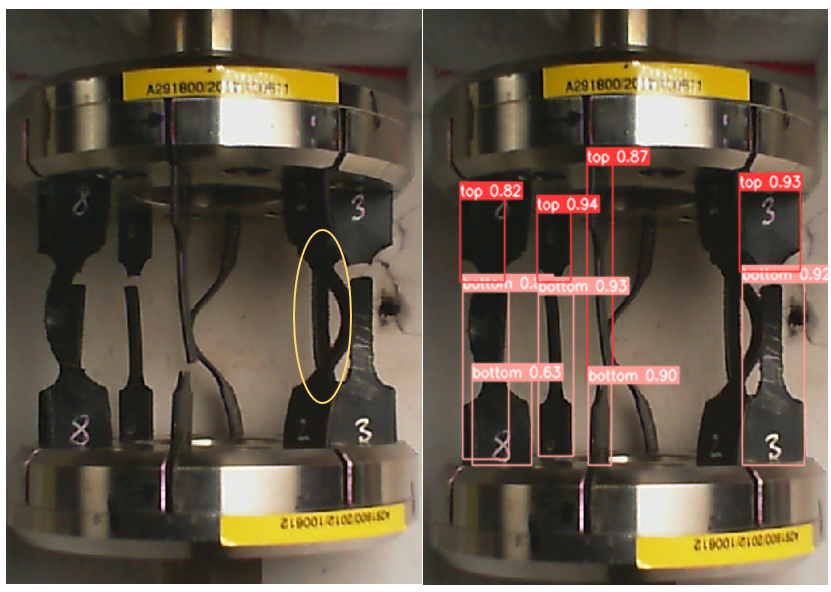
\includegraphics[width=0.75\textwidth]{gfx/image_1.png}
 \caption{Die gelb markierte Probe wird von der vorderen Probe überlappt und sieht daher aus, als wäre sie nicht gerissen. Das führt dazu, dass sie nicht von YOLO erkannt wird}
 \label{fig:part01:image_1}
\end{figure}

\begin{figure}[!htbp]
 \centering
 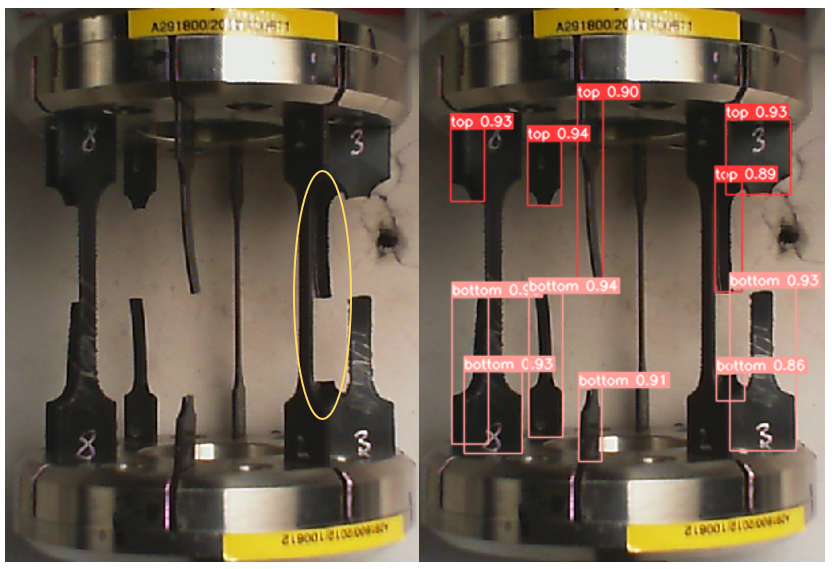
\includegraphics[width=0.75\textwidth]{gfx/image_2.png}
 \caption{Die gelb markierte Probe ist in dieser Phase wieder erkennbar}
 \label{fig:part01:image_2}
\end{figure}

Um dieses Problem zu lösen, haben wir eine Lösung entwickelt: Wir definieren eine Mittellinie zwischen den Einspannungen und setzen eine Tracking-Grenze fest. Wenn die Proben sehr stark gestaucht sind, d.h. die Mittellinie zwischen den Einspannungen die Tracking-Grenze überschreitet­­­, wird der Tracker gestoppt. Dies verhindert Überlappungen und minimiert den Wechsel in den Objekt-IDs. Die Berechnung der Mittellinie (mL) erfolgt in \ref{eq:part01:middle_line}.

\begin{gather}
mL = \frac{\frac{\sum_{i=1}^{n} (y_i - \frac{h_i}{2})}{n} + \frac{\sum_{j=1}^{m} (y_i + \frac{h_j}{2})}{m}}{2}
\label{eq:part01:middle_line}
\end{gather}

\begin{align*}
& \text{Mit:} \\
& - n: \text{ist die Anzahl von Bounding Boxen mit "Top" Klasse} \\
& - m: \text{ist die Anzahl von Bounding Boxen mit "Bottom" Klasse} \\
& - y_i: \text{y Wert vom Mittelpunkt des Bounding Box i} \\
& - h_i: \text{die Höhe des Bounding Box i}
\end{align*}

Im Bild \ref{fig:part01:image_3} sehen wir die blau markierte Mittellinie im linken Bild, die sich unterhalb der Tracking-Grenze (grün) befindet. Aus diesem Grund ordnet der Tracker die von Detector erkannten Objekte einer ID zu. Im rechten Bild hingegen befindet sich die Mittellinie oberhalb der Tracking-Grenze, weshalb der Tracker stoppt und somit kein Objekt einer ID zugeordnet wird.

\begin{figure}[htbp]
 \centering
 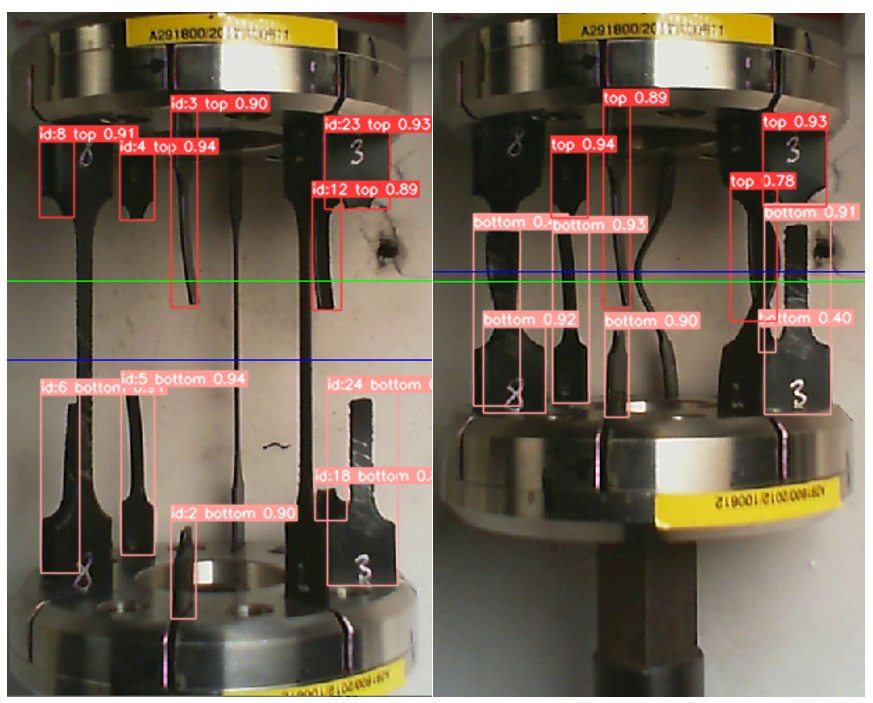
\includegraphics[width=0.8\textwidth]{gfx/image_3.png}
 \caption{Links: Tracker funkioniert. Rechts: Tracker pausiert}
 \label{fig:part01:image_3}
\end{figure}

Um diesen Punkt zu verdeutlichen, haben wir die Performance des Trackings sowohl mit als auch ohne die Verwendung der Tracking-Grenze für ein Video gemessen. Die Heatmap in \ref{fig:part01:image_4} zeigt, dass eine Region rot markiert wird, wenn ein ID-Wechsel in diesem Bereich auftritt. Wir sehen, dass im Fall des Trackings mit Tracking-Grenze (linkes Bild) lediglich eine Probe mit einem ID-Wechsel vorhanden ist, während beim Tracking ohne Tracking-Grenze (rechtes Bild) insgesamt vier Proben ID-Wechsel aufweisen. Die Tabelle \ref{tab:Tracking_performance} zeigt, dass die Einführung der Tracking-Grenze  zu einer erheblichen Reduzierung der Anzahl von ID-Wechseln, \acs{FP}, \acs{FN} führte, was wiederum das \acs{MOTA} des Trackings erheblich verbesserte. 

\begin{figure}[htbp]
 \centering
 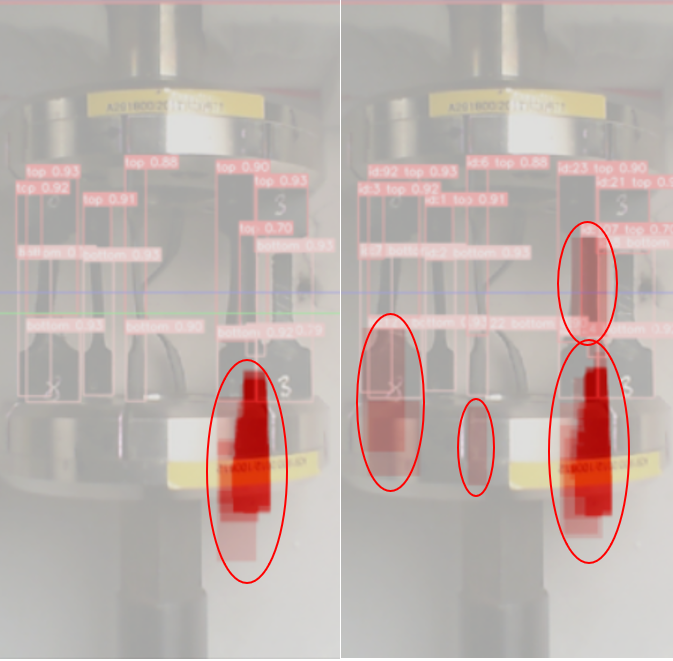
\includegraphics[width=0.8\textwidth]{gfx/image_4.png}
 \caption{Links: Tracking mit Tracking-Grenze hat ID-Wechsel nur bei einer Probe. Rechts: Tracking ohne Tracking-Grenze hat ID-Wechsel bei 4 Proben.}
 \label{fig:part01:image_4}
\end{figure}

\begin{table}[htbp]
    \myfloatalign
    \begin{tabular}{ccccc} 
            \tableheadline{Art des Tracking} & 
            \tableheadline{FN} & 
            \tableheadline{FP} &
            \tableheadline{ID-Wechsel} &
            \tableheadline{MOTA}\\ 
        \midrule
            Ohne Tracking-Grenze & 248 & 159 & 76 & 88.76\% \\
            Mit Tracking-Grenze  & 51  & 40  & 35 & 94.32\%
    \end{tabular}
    \caption{Tracking's Performance mit und ohne Tracking-Grenze.}
    \label{tab:Tracking_performance}
\end{table}
    